\documentclass[10pt,aspectratio=169]{beamer}

%================================================
% Theme
%================================================
\usetheme[numbering=fraction,progressbar=frametitle]{metropolis}
\metroset{sectionpage=none}

%================================================
% Packages
%================================================
\usepackage{amsmath,amssymb}
\usepackage{booktabs}
\usepackage{tikz}
\usetikzlibrary{automata,positioning,arrows.meta,calc,trees}
\usepackage{xcolor}
\usepackage{listings}

%================================================
% Metadata
%================================================
\newcommand{\LastCompiled}{\today}

\title{Theory of Computation}
\subtitle{Lecture 5: Regular Operations and Regular Expressions}
\author{Sheikh Azizul Hakim\\Lecturer, Department of CSE, BUET}
\date{Last compiled: \LastCompiled}

%================================================
% Listings
%================================================
\lstdefinestyle{code}{
  basicstyle=\ttfamily\small,
  frame=single,
  backgroundcolor=\color{black!4},
  rulecolor=\color{black!20},
  showstringspaces=false,
  columns=fullflexible,
  keepspaces=true
}
\lstset{style=code}

%================================================
% Helpers
%================================================
\newcommand{\eps}{\varepsilon}
\newcommand{\powset}[1]{\mathcal P({#1})}
\newcommand{\lang}[1]{\mathsf{#1}}

\tikzset{
  every state/.style={minimum size=8mm},
  >=Stealth,
  shorten >=1pt,
}

%================================================
\begin{document}

%================================================
\maketitle

%================================================
\begin{frame}[standout]
We have machines that compute.

Now we need an algebra to describe what they compute.
\end{frame}


%------------------------------------------------
\begin{frame}{Today's Roadmap}

This lecture follows the central arc of Sipser's treatment of regular languages.

\vspace{0.7em}
\begin{enumerate}
    \item Define the three \textbf{regular operations}.
    \item Prove regular languages are closed under them.
    \item Define \textbf{regular expressions} formally.
    \item Prove that regular expressions and finite automata have exactly the same power.
\end{enumerate}

\vspace{0.7em}
The goal is not just to memorize constructions, but to see one idea repeat:
\[
\text{language operation} \quad \Longleftrightarrow \quad \text{machine construction}.
\]

\end{frame}


%================================================
\section{Lecture 5A: The Regular Operations}

%------------------------------------------------
\begin{frame}{Languages as Sets}

Recall that a \textbf{language} is simply a set of strings.

\vspace{1em}

Because languages are sets, we can combine them using set operations to build new, more complex languages.

\vspace{1em}

In automata theory, three specific operations are fundamental. We call these the \textbf{regular operations}.

\end{frame}


%------------------------------------------------
\begin{frame}{Alphabet, Strings, and Languages}

Fix an alphabet $\Sigma$.

\vspace{0.7em}
\begin{table}
\centering
\begin{tabular}{ll}
\toprule
\textbf{Object} & \textbf{Meaning} \\
\midrule
$\Sigma$ & a finite set of symbols \\
$w$ & a finite string over $\Sigma$ \\
$\eps$ & the empty string \\
$\Sigma^*$ & the set of all strings over $\Sigma$ \\
$A \subseteq \Sigma^*$ & a language over $\Sigma$ \\
\bottomrule
\end{tabular}
\end{table}

\vspace{0.7em}
A regular operation takes one or more languages and returns another language.

\end{frame}

%------------------------------------------------
\begin{frame}{Operations on Languages Are Not Operations on Machines}

When we write $A \cup B$, $AB$, or $A^*$, we are talking about sets of strings.

\vspace{0.8em}
The machine comes later.

\vspace{0.8em}
\begin{center}
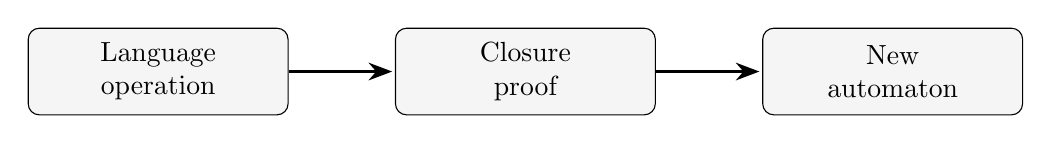
\begin{tikzpicture}[
  box/.style={draw, rounded corners, fill=black!4, minimum width=3.3cm, minimum height=1.1cm, align=center},
  arr/.style={-{Stealth[length=3mm]}, thick}
]
  \node[box] (op) {Language\\operation};
  \node[box, right=1.35cm of op] (proof) {Closure\\proof};
  \node[box, right=1.35cm of proof] (mach) {New\\automaton};
  \draw[arr] (op) -- (proof);
  \draw[arr] (proof) -- (mach);
\end{tikzpicture}
\end{center}

\vspace{0.8em}
Closure proofs answer the question: if the inputs have machines, can we build a machine for the output language?

\end{frame}

%------------------------------------------------
\begin{frame}{The Three Regular Operations}

Let $A$ and $B$ be languages. We define the regular operations as follows:

\vspace{1em}

\begin{enumerate}
    \item \textbf{Union:} $A \cup B = \{x \mid x \in A \text{ or } x \in B\}$
    \vspace{0.5em}
    \item \textbf{Concatenation:} $A \circ B = \{xy \mid x \in A \text{ and } y \in B\}$
    \vspace{0.5em}
    \item \textbf{Star:} $A^* = \{x_1x_2\dots x_k \mid k \geq 0 \text{ and each } x_i \in A\}$
\end{enumerate}

\end{frame}

%------------------------------------------------
\begin{frame}{Understanding Union}

\textbf{Definition:} $A \cup B = \{x \mid x \in A \text{ or } x \in B\}$

\vspace{1em}

The union simply takes all strings from $A$ and all strings from $B$ and puts them into a single set.

\vspace{1em}

\textbf{Example:}
Let $\Sigma = \{a, b\}$.
\begin{align*}
A &= \{\text{good}, \text{bad}\} \\
B &= \{\text{boy}, \text{girl}\}
\end{align*}

$$A \cup B = \{\text{good}, \text{bad}, \text{boy}, \text{girl}\}$$

\end{frame}

%------------------------------------------------
\begin{frame}{Understanding Concatenation}

\textbf{Definition:} $A \circ B = \{xy \mid x \in A \text{ and } y \in B\}$

\vspace{1em}

Concatenation attaches a string from $A$ to the front of a string from $B$ in all possible combinations.

\vspace{1em}

\textbf{Example:}
Let $A = \{\text{good}, \text{bad}\}$ and $B = \{\text{boy}, \text{girl}\}$.

\vspace{0.5em}
$$A \circ B = \{\text{goodboy}, \text{goodgirl}, \text{badboy}, \text{badgirl}\}$$

\vspace{1em}
\pause
\textit{Note: We often omit the circle and just write $AB$.}

\end{frame}

%------------------------------------------------
\begin{frame}{Understanding Kleene Star}

\textbf{Definition:} $A^* = \{x_1x_2\dots x_k \mid k \geq 0 \text{ and each } x_i \in A\}$

\vspace{1em}

The star operation is a \textbf{unary} operation. It attaches any number of strings in $A$ together to get a new string.

\vspace{0.5em}
Because $k$ can be $0$, the empty string $\eps$ is \textbf{always} in $A^*$, regardless of what $A$ is.

\vspace{1em}

\textbf{Example:}
Let $A = \{ab, c\}$.

$$A^* = \{\eps, ab, c, abab, abc, cab, cc, ababab, ababc, \dots\}$$

\end{frame}


%------------------------------------------------
\begin{frame}{Why Star Always Contains $\eps$}

For a language $A$, the expression $A^*$ means concatenate \textbf{zero or more} strings from $A$.

\vspace{0.8em}
If we concatenate zero strings, the result is the empty string:
\[
A^* = \{\eps\} \cup A \cup AA \cup AAA \cup \cdots
\]

\vspace{0.8em}
So:
\[
\eps \in A^* \quad \text{for every language } A.
\]

\pause
\vspace{0.6em}
This is why $\emptyset^* = \{\eps\}$, not $\emptyset$.

\end{frame}

%------------------------------------------------
\begin{frame}{Regular Languages}

\textbf{Definition:} A language is called a \textbf{regular language} if some DFA recognizes it.

\vspace{1em}

\textbf{Alternative Definition:} A language is called a \textbf{regular language} if some NFA recognizes it.

\vspace{1em}

Both are valid since a DFA is trivially an NFA and every NFA has an equivalent DFA.
\vspace{1em}
\pause

\textbf{The Big Question:} 
If we take two regular languages and apply a regular operation to them, is the resulting language still regular?

\end{frame}


%------------------------------------------------
\begin{frame}{Sipser's Closure Theorem}

Sipser proves the following theorem early because it becomes the bridge to regular expressions.

\vspace{0.8em}
\textbf{Theorem.} The class of regular languages is closed under the regular operations:
\[
\cup,\qquad \circ,\qquad ^*.
\]

\vspace{0.8em}
\pause
The proof uses NFAs because $\eps$-transitions make the constructions visually and formally simple.

\vspace{0.8em}
This is also why nondeterminism is not a side topic; it is the cleanest language-design tool we have.

\end{frame}

%================================================
\section{Lecture 5B: Closure Properties}

%------------------------------------------------
\begin{frame}{What is a Closure Property?}

A collection of objects is \textbf{closed} under some operation if applying that operation to members of the collection returns an object still in the collection.

\vspace{1em}

\textbf{Mathematical Examples:}
\begin{itemize}
    \item The set of natural numbers $\mathbb{N}$ is closed under addition. \\ ($3 + 5 = 8 \in \mathbb{N}$)
    \item $\mathbb{N}$ is \textbf{not} closed under subtraction. \\ ($3 - 5 = -2 \notin \mathbb{N}$)
\end{itemize}

\end{frame}

%------------------------------------------------
\begin{frame}{Closure of Regular Languages}

\textbf{Theorem:} The class of regular languages is closed under the union operation.

\vspace{1em}

In other words, if $A_1$ and $A_2$ are regular languages, then $A_1 \cup A_2$ is also a regular language.

\vspace{1em}
\pause

\textbf{Proof Idea:} 
Since $A_1$ and $A_2$ are regular, there exist machines $M_1$ and $M_2$ that recognize them. We must build a new machine $M$ that recognizes $A_1 \cup A_2$.

\end{frame}

%------------------------------------------------
\begin{frame}{Building the Union Machine}

How does $M$ accept an input $w$?
It should accept if either $M_1$ accepts $w$ or $M_2$ accepts $w$.

\vspace{1em}

We \textit{could} build a DFA that simulates $M_1$ and $M_2$ simultaneously (keeping track of pairs of states). 

\vspace{1em}
\pause
But remember our new tool: \textbf{Nondeterminism}.

With an NFA, we can just \textit{guess} which machine will accept!

\end{frame}

%------------------------------------------------
\begin{frame}{Proof: Closure under Union}
\small

Let $N_1$ recognize $A_1$ and $N_2$ recognize $A_2$.
We construct a new NFA $N$ to recognize $A_1 \cup A_2$.

\begin{center}
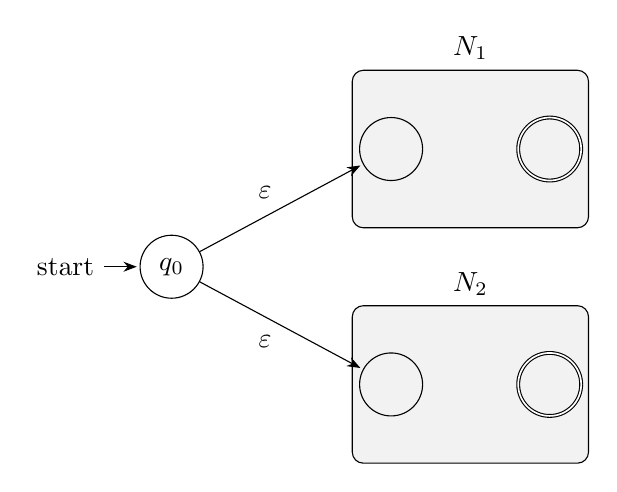
\begin{tikzpicture}[
  ->,>=Stealth,shorten >=1pt,
  node distance=2.5cm,
  every state/.style={minimum size=8mm},
  box/.style={draw, rounded corners, minimum width=3cm, minimum height=2cm, fill=black!5}
]

\node[state, initial] (q0) {$q_0$};

\node[box, above right=0.2cm and 2cm of q0] (M1) {};
\node[state] (start1) at (M1.west) [xshift=0.5cm] {};
\node[state, accepting] (acc1) at (M1.east) [xshift=-0.5cm] {};
\node[above] at (M1.north) {$N_1$};

\node[box, below right=0.2cm and 2cm of q0] (M2) {};
\node[state] (start2) at (M2.west) [xshift=0.5cm] {};
\node[state, accepting] (acc2) at (M2.east) [xshift=-0.5cm] {};
\node[above] at (M2.north) {$N_2$};

\path
(q0) edge node[above left] {$\eps$} (start1)
(q0) edge node[below left] {$\eps$} (start2);

\end{tikzpicture}
\end{center}

\vspace{0.3em}
Add a new start state $q_0$ and $\eps$-transitions to the start states of $N_1$ and $N_2$.

\end{frame}


%------------------------------------------------
\begin{frame}{Union Construction: Formal Version}

Let
\[
N_1=(Q_1,\Sigma,\delta_1,q_1,F_1),\qquad
N_2=(Q_2,\Sigma,\delta_2,q_2,F_2)
\]
recognize $A_1$ and $A_2$.

\vspace{0.7em}
Construct $N=(Q,\Sigma,\delta,q_0,F)$ where:
\begin{align*}
Q &= Q_1 \cup Q_2 \cup \{q_0\},\\
F &= F_1 \cup F_2.
\end{align*}

\vspace{0.5em}
The new transition function keeps all old transitions and adds:
\[
\delta(q_0,\eps)=\{q_1,q_2\}.
\]

\end{frame}

%------------------------------------------------
\begin{frame}{Closure under Concatenation}

\textbf{Theorem:} The class of regular languages is closed under the concatenation operation.

\vspace{1em}

If $A_1$ and $A_2$ are regular, then $A_1 \circ A_2$ is regular.

\vspace{1em}
\pause

\textbf{Proof Idea:} 
Given string $w$, we want to split it into $w = xy$ such that $x \in A_1$ and $y \in A_2$. 
But we don't know where the split point is!

\vspace{1em}
\textbf{NFA to the rescue:} We guess the split point.

\end{frame}

%------------------------------------------------
\begin{frame}{Proof: Closure under Concatenation}

Let $N_1$ recognize $A_1$ and $N_2$ recognize $A_2$.
We construct $N$ to recognize $A_1 \circ A_2$.

\onslide<1>{
\begin{center}
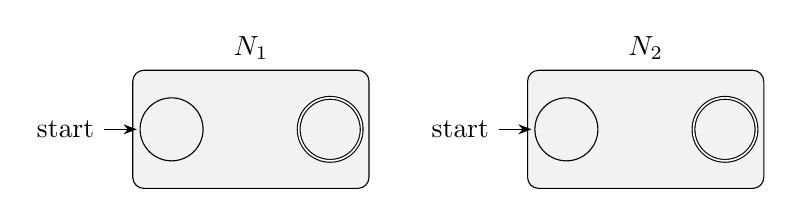
\begin{tikzpicture}[
  ->,>=Stealth,shorten >=1pt,
  node distance=2.5cm,
  every state/.style={minimum size=8mm},
  box/.style={draw, rounded corners, minimum width=3cm, minimum height=1.5cm, fill=black!5}
]

\node[box] (M1) {};
\node[state, initial] (start1) at (M1.west) [xshift=0.5cm] {};
\node[state, accepting] (acc1) at (M1.east) [xshift=-0.5cm] {};
\node[above] at (M1.north) {$N_1$};

\node[box, right=2cm of M1] (M2) {};
\node[state, initial] (start2) at (M2.west) [xshift=0.5cm] {};
\node[state, accepting] (acc2) at (M2.east) [xshift=-0.5cm] {};
\node[above] at (M2.north) {$N_2$};


\end{tikzpicture}
\end{center}
}
{
\begin{center}
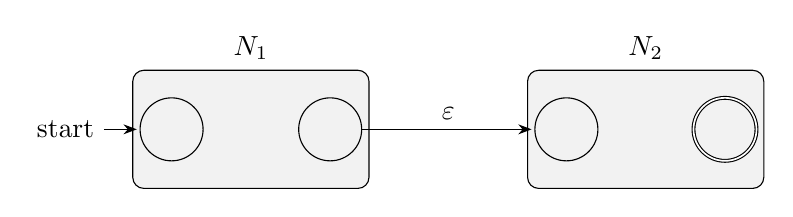
\begin{tikzpicture}[
  ->,>=Stealth,shorten >=1pt,
  node distance=2.5cm,
  every state/.style={minimum size=8mm},
  box/.style={draw, rounded corners, minimum width=3cm, minimum height=1.5cm, fill=black!5}
]

\node[box] (M1) {};
\node[state, initial] (start1) at (M1.west) [xshift=0.5cm] {};
\node[state] (acc1) at (M1.east) [xshift=-0.5cm] {};
\node[above] at (M1.north) {$N_1$};

\node[box, right=2cm of M1] (M2) {};
\node[state] (start2) at (M2.west) [xshift=0.5cm] {};
\node[state, accepting] (acc2) at (M2.east) [xshift=-0.5cm] {};
\node[above] at (M2.north) {$N_2$};

\path
(acc1) edge node[above] {$\eps$} (start2);

\end{tikzpicture}
\end{center}
}
\vspace{0.3em}
Connect all accepting states of $N_1$ to the start state of $N_2$ using $\eps$-transitions. The accept states of $N_1$ are no longer accepting.

\end{frame}


%------------------------------------------------
\begin{frame}{Concatenation Construction: Formal Version}

Let $N_1$ recognize $A_1$ and $N_2$ recognize $A_2$.

\vspace{0.8em}
The new NFA starts in the start state of $N_1$ and accepts in the accepting states of $N_2$.

\vspace{0.8em}
The key added transitions are:
\[
\delta(r,\eps) \ni q_2 \quad \text{for every } r \in F_1,
\]
where $q_2$ is the start state of $N_2$.

\vspace{0.8em}
Interpretation: after reading some prefix $x\in A_1$, the machine may jump into $N_2$ and try to read the remaining suffix $y\in A_2$.

\end{frame}

%------------------------------------------------
\begin{frame}{Concatenation: Why Nondeterminism Is Natural}

For $A_1A_2$, the machine must decide where the first part ends.

\vspace{0.8em}
Example:
\[
w=001101
\]
Maybe $w=00\,1101$, or $w=001\,101$, or $w=0011\,01$.

\vspace{0.8em}
A DFA can simulate all possibilities indirectly, but the NFA construction says the idea directly:

\vspace{0.6em}
\begin{center}
\textit{At an accepting state of $N_1$, guess that the split point is here.}
\end{center}

\end{frame}

%------------------------------------------------
\begin{frame}{Closure under Star}

\textbf{Theorem:} The class of regular languages is closed under the star operation.

\vspace{1em}

If $A$ is regular, then $A^*$ is regular.

\vspace{1em}
\pause

\textbf{Proof Idea:} 
We have a machine $N_1$ for $A$. To accept $A^*$, the machine must accept sequences of strings from $A$. 

When $N_1$ finishes reading one string in $A$, it should non-deterministically jump back to the beginning to start reading the next string.

\end{frame}

%------------------------------------------------
\begin{frame}{Proof: Closure under Star}

We must also accept $\eps$, so we add a new accepting start state.

\begin{center}
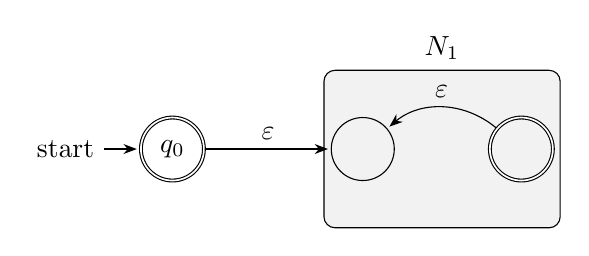
\begin{tikzpicture}[
  ->,>=Stealth,shorten >=1pt,
  node distance=2.5cm,
  every state/.style={minimum size=8mm},
  box/.style={draw, rounded corners, minimum width=3cm, minimum height=2cm, fill=black!5}
]

\node[state, initial, accepting] (q0) {$q_0$};

\node[box, right=1.5cm of q0] (M1) {};
\node[state] (start1) at (M1.west) [xshift=0.5cm] {};
\node[state, accepting] (acc1) at (M1.east) [xshift=-0.5cm] {};
\node[above] at (M1.north) {$N_1$};

\path
(q0) edge node[above] {$\eps$} (start1)
(acc1) edge[bend right=40] node[above] {$\eps$} (start1);

\end{tikzpicture}
\end{center}

\vspace{0.3em}
Add new start state $q_0$, an $\eps$-arrow to the old start state, and $\eps$-arrows from all old accept states back to the old start state.

\end{frame}


%------------------------------------------------
\begin{frame}{Star Construction: Formal Version}

Let $N_1=(Q_1,\Sigma,\delta_1,q_1,F_1)$ recognize $A$.

\vspace{0.8em}
Create a new start state $q_0$ that is also accepting. Then:
\[
Q = Q_1 \cup \{q_0\}, \qquad F = F_1 \cup \{q_0\}.
\]

\vspace{0.8em}
Add:
\[
\delta(q_0,\eps) \ni q_1
\]
and for every $r\in F_1$:
\[
\delta(r,\eps) \ni q_1.
\]

\vspace{0.8em}
The new accepting start state accounts for the case of zero repetitions.

\end{frame}

%------------------------------------------------
\begin{frame}{A Closure Proof Template}

Most closure proofs have the same rhythm.

\vspace{0.8em}
\begin{enumerate}
    \item Start with machines for the input languages.
    \item Describe the language operation we want to simulate.
    \item Build a new finite automaton.
    \item Argue both directions: every accepted string belongs to the target language, and every target string is accepted.
\end{enumerate}

\vspace{0.8em}
For regular operations, the construction is usually the heart of the proof.

\end{frame}

%------------------------------------------------
\begin{frame}{Two Directions in a Correctness Proof}

For a constructed machine $N$ and target language $L$, we prove:

\vspace{0.8em}
\begin{align*}
L(N) \subseteq L &\quad \text{(machine accepts nothing extra)},\\
L \subseteq L(N) &\quad \text{(machine accepts everything required)}.
\end{align*}

\vspace{0.8em}
Example for union: if $N$ accepts $w$, some branch went into $N_1$ or $N_2$; if $w\in A_1\cup A_2$, choose the branch for the accepting machine.

\end{frame}

%------------------------------------------------
\begin{frame}[standout]
Because the class of regular languages is closed under Union, Concatenation, and Star, we can use these operations as a toolkit to build any regular language.
\end{frame}

%================================================
% INSERT THESE FRAMES AT THE END OF SECTION 6B, 
% Extended closure material before the regular-expression section
%================================================

%------------------------------------------------
\begin{frame}[standout]
Union, Concatenation, and Star are the ``Regular Operations''.

But regular languages are closed under many other operations too.
\end{frame}

%------------------------------------------------
\begin{frame}{Closure under Complement}

\textbf{Definition:} The complement of a language $A$, denoted $\overline{A}$, is the set of all strings in $\Sigma^*$ that are \textbf{not} in $A$.
\[
\overline{A} = \Sigma^* \setminus A
\]

\vspace{1em}
\textbf{Theorem:} The class of regular languages is closed under complement.

\vspace{1em}
\pause
\textbf{Proof Idea:} 
If $A$ is regular, there is a machine $M$ that recognizes it. To build a machine that recognizes $\overline{A}$, we just run $M$ and do the exact opposite of what it does.

If $M$ accepts, we reject. If $M$ rejects, we accept.

\end{frame}

%------------------------------------------------
\begin{frame}{Proof: Closure under Complement}

Let $M = (Q, \Sigma, \delta, q_0, F)$ be a \textbf{DFA} recognizing $A$.

\vspace{1em}

We construct a new DFA $M' = (Q, \Sigma, \delta, q_0, F')$ recognizing $\overline{A}$.

\vspace{1em}

The only difference is the set of accepting states:
\[
F' = Q \setminus F
\]

\vspace{1em}
\pause
\textbf{Warning!} This construction \textbf{only works for DFAs}. 
If you flip the accept states of an NFA, the new NFA does not necessarily recognize the complement. (Why? Because an NFA accepts if \textit{any} path reaches an accept state. Flipping states doesn't invert this logic correctly).

\end{frame}


%------------------------------------------------
\begin{frame}{Complement Requires a Complete DFA}

The complement construction assumes that every input string follows exactly one full computation path.

\vspace{0.8em}
So before flipping accepting states, make sure the DFA is \textbf{complete}:
\[
\delta(q,a) \text{ is defined for every } q\in Q \text{ and } a\in\Sigma.
\]

\vspace{0.8em}
If a transition is missing, add a dead state and send the missing transition there.

\vspace{0.8em}
This small detail prevents a common mistake: rejection by ``getting stuck'' is not the same as ending in a nonaccepting state unless the automaton model says so explicitly.

\end{frame}

%------------------------------------------------
\begin{frame}{Example: Complementing a DFA}
\small

Language $A$: Strings ending in $0$.

\textbf{Original DFA ($M$):}
\begin{center}
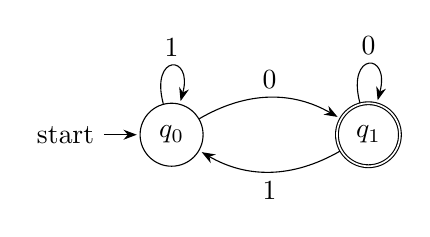
\begin{tikzpicture}[
  ->,>=Stealth,shorten >=1pt,
  node distance=2.5cm,
  every state/.style={minimum size=8mm},
]
\node[state, initial] (q0) {$q_0$};
\node[state, accepting, right of=q0] (q1) {$q_1$};

\path 
(q0) edge[bend left] node[above] {$0$} (q1)
(q0) edge[loop above] node {$1$} ()
(q1) edge[bend left] node[below] {$1$} (q0)
(q1) edge[loop above] node {$0$} ();
\end{tikzpicture}
\end{center}

\vspace{0.5em}
Language $\overline{A}$: $\eps$ or strings ending in $1$.

\textbf{Complemented DFA ($M'$):}
\begin{center}
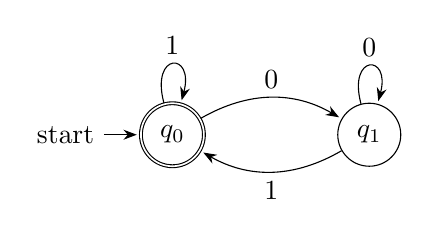
\begin{tikzpicture}[
  ->,>=Stealth,shorten >=1pt,
  node distance=2.5cm,
  every state/.style={minimum size=8mm},
]
\node[state, initial, accepting] (q0) {$q_0$};
\node[state, right of=q0] (q1) {$q_1$};

\path 
(q0) edge[bend left] node[above] {$0$} (q1)
(q0) edge[loop above] node {$1$} ()
(q1) edge[bend left] node[below] {$1$} (q0)
(q1) edge[loop above] node {$0$} ();
\end{tikzpicture}
\end{center}

\end{frame}

%------------------------------------------------
\begin{frame}{Closure under Intersection}

\textbf{Definition:} $A \cap B = \{x \mid x \in A \text{ and } x \in B\}$

\vspace{1em}
\textbf{Theorem:} The class of regular languages is closed under intersection.

\vspace{1em}
\pause
There are two beautiful ways to prove this:
\begin{enumerate}
    \item \textbf{Constructive Proof (Product Construction):} Build a machine that runs $M_1$ and $M_2$ simultaneously.
    \item \textbf{Algebraic Proof:} Use De Morgan's Laws.
\end{enumerate}

\end{frame}

%------------------------------------------------
\begin{frame}{Intersection Proof 1: Product Construction}

Let $M_1 = (Q_1, \Sigma, \delta_1, q_1, F_1)$ and $M_2 = (Q_2, \Sigma, \delta_2, q_2, F_2)$ be DFAs.

\vspace{1em}
We build $M = (Q, \Sigma, \delta, q_0, F)$ to simulate both.
The states of $M$ are pairs of states from $M_1$ and $M_2$.

\vspace{1em}
\begin{itemize}
    \item \textbf{States:} $Q = Q_1 \times Q_2 = \{(r_1, r_2) \mid r_1 \in Q_1 \text{ and } r_2 \in Q_2\}$
    \item \textbf{Start state:} $q_0 = (q_1, q_2)$
    \item \textbf{Transitions:} $\delta((r_1, r_2), a) = (\delta_1(r_1, a), \delta_2(r_2, a))$
\end{itemize}

\vspace{1em}
\pause
To accept $A \cap B$, \textbf{both} machines must accept.
Therefore:
\[
F = \{(r_1, r_2) \mid r_1 \in F_1 \textbf{ and } r_2 \in F_2\} = F_1 \times F_2
\]

\end{frame}


%------------------------------------------------
\begin{frame}{Reading Product States}

In the product construction, a state $(r,s)$ means:

\vspace{0.7em}
\begin{center}
After reading the same input prefix, $M_1$ is in state $r$ and $M_2$ is in state $s$.
\end{center}

\vspace{0.8em}
This is the finite-automata version of running two programs side by side.

\vspace{0.8em}
For intersection, a product state is accepting only when both coordinates are accepting.

\[
(r,s)\in F \quad \Longleftrightarrow \quad r\in F_1 \text{ and } s\in F_2.
\]

\end{frame}

%------------------------------------------------
\begin{frame}{Intersection Proof 2: De Morgan's Laws}

A faster way to prove closure under intersection relies on what we already know.

\vspace{1em}
Recall De Morgan's Law for sets:
\[
A \cap B = \overline{\overline{A} \cup \overline{B}}
\]

\vspace{1em}
\pause
We already proved that regular languages are closed under:
\begin{itemize}
    \item \textbf{Complement} ($\overline{A}$ and $\overline{B}$ are regular)
    \item \textbf{Union} ($\overline{A} \cup \overline{B}$ is regular)
    \item \textbf{Complement again} ($\overline{\overline{A} \cup \overline{B}}$ is regular)
\end{itemize}

\vspace{1em}
Therefore, $A \cap B$ must be regular. No new machines to build!

\end{frame}

%------------------------------------------------
\begin{frame}{Closure under Difference}

\textbf{Definition:} $A \setminus B = \{x \mid x \in A \text{ and } x \notin B\}$

\vspace{1em}
\textbf{Theorem:} The class of regular languages is closed under set difference.

\vspace{1em}
\pause
\textbf{Proof:}
Notice that $A \setminus B$ is simply the intersection of $A$ and the complement of $B$.

\[
A \setminus B = A \cap \overline{B}
\]

Since regular languages are closed under complement and intersection, they are closed under difference.

\end{frame}

%------------------------------------------------
\begin{frame}{Closure under Reverse}

\textbf{Definition:} The reverse of a string $w = c_1c_2\dots c_n$ is $w^R = c_n\dots c_2c_1$.
The reverse of a language $A$ is $A^R = \{w^R \mid w \in A\}$.

\vspace{1em}
\textbf{Theorem:} The class of regular languages is closed under reversal.

\vspace{1em}
\pause
\textbf{Proof Idea:} 
If $M$ is a machine that accepts a string by reading it forwards, we can build a new machine $M^R$ that accepts by reading the string backwards. 

To do this, we just reverse all the arrows in the transition diagram of $M$.

\end{frame}

%------------------------------------------------
\begin{frame}{Building the Reverse Machine}

Take a DFA $M$ that recognizes $A$. We build an NFA $N$ to recognize $A^R$.

\vspace{1em}
\begin{enumerate}
    \item Reverse the direction of every transition arrow.
    \item The old start state becomes the new \textbf{single accept state}.
    \item Create a \textbf{new start state}.
    \item Draw $\eps$-transitions from the new start state to all of the old accept states.
\end{enumerate}

\vspace{1em}
\pause
Why an NFA? 
Reversing arrows can turn a deterministic machine into a nondeterministic one (e.g., two arrows with the same symbol might now leave a state).

\end{frame}

%------------------------------------------------
\begin{frame}{Visualizing Reversal}
\small

\textbf{Original DFA for $A$:}
\begin{center}
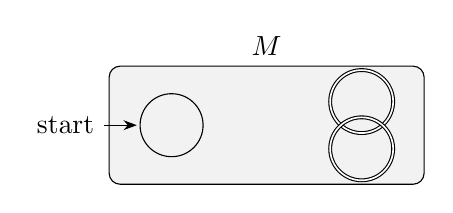
\begin{tikzpicture}[
  ->,>=Stealth,shorten >=1pt,
  node distance=2.5cm,
  every state/.style={minimum size=8mm},
  box/.style={draw, rounded corners, minimum width=4cm, minimum height=1.5cm, fill=black!5}
]
\node[box] (M) {};
\node[state, initial] (start) at (M.west) [xshift=0.8cm] {};
\node[state, accepting] (acc1) at (M.east) [xshift=-0.8cm, yshift=0.3cm] {};
\node[state, accepting] (acc2) at (M.east) [xshift=-0.8cm, yshift=-0.3cm] {};
\node[above] at (M.north) {$M$};
\end{tikzpicture}
\end{center}

\vspace{0.5em}
\textbf{Reversed NFA for $A^R$:}
\begin{center}
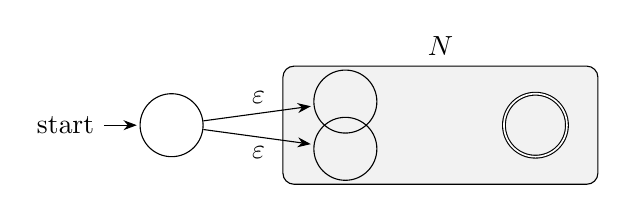
\begin{tikzpicture}[
  ->,>=Stealth,shorten >=1pt,
  node distance=2.5cm,
  every state/.style={minimum size=8mm},
  box/.style={draw, rounded corners, minimum width=4cm, minimum height=1.5cm, fill=black!5}
]
\node[box] (M) {};
\node[state, accepting] (oldstart) at (M.east) [xshift=-0.8cm] {};
\node[state] (oldacc1) at (M.west) [xshift=0.8cm, yshift=0.3cm] {};
\node[state] (oldacc2) at (M.west) [xshift=0.8cm, yshift=-0.3cm] {};
\node[state, initial, left=1cm of M.west] (newstart) {};

\path 
(newstart) edge node[above] {$\eps$} (oldacc1)
(newstart) edge node[below] {$\eps$} (oldacc2);
\node[above] at (M.north) {$N$};
\end{tikzpicture}
\end{center}
\vspace{0.3em}
\small (Assume all internal arrows inside the box are reversed).

\end{frame}

%------------------------------------------------
\begin{frame}{The Power of Closure Properties}

By knowing these closure properties, we can prove languages are regular without ever drawing a state diagram!

\vspace{1em}
\textbf{Example:} Let $L$ be the language of strings over $\{0,1\}$ that contain $101$ but do \textbf{not} end in $11$. Is $L$ regular?

\vspace{1em}
\pause
Yes.
\begin{itemize}
    \item $L_1 = \{w \mid w \text{ contains } 101\}$ is regular (we built a DFA for it).
    \item $L_2 = \{w \mid w \text{ ends in } 11\}$ is regular.
    \item $L = L_1 \setminus L_2$.
\end{itemize}
Since regular languages are closed under set difference, $L$ is regular.

\end{frame}


%------------------------------------------------
\begin{frame}{Closure as a Proof Shortcut}

Closure properties let us avoid building large automata manually.

\vspace{0.8em}
Suppose $A$ is the language of strings over $\{0,1\}$ that contain $101$, and $B$ is the language of strings that have even length.

\vspace{0.8em}
Then the language
\[
A \cap B
\]
is regular because both $A$ and $B$ are regular and regular languages are closed under intersection.

\vspace{0.8em}
The proof is modular: prove small components regular, then combine them.

\end{frame}

%================================================
\section{Lecture 5C: Regular Expressions}

%------------------------------------------------
\begin{frame}{What is a Regular Expression?}

We can use the regular operations to build up expressions describing languages, just as we use arithmetic operations ($+, \times$) to build up expressions describing numbers.

\vspace{1em}

\textbf{Arithmetic Example:} $(5 + 3) \times 4$ evaluates to $32$.

\vspace{1em}

\textbf{Language Example:} $(0 \cup 1) 0^*$ evaluates to the language of all strings starting with a $0$ or a $1$, followed by any number of $0$s.

\vspace{1em}
\pause
These expressions are called \textbf{Regular Expressions (RE)}.

\end{frame}


%------------------------------------------------
\begin{frame}{Syntax Versus Semantics}

A regular expression is a piece of syntax.

\vspace{0.8em}
Its meaning is a language.

\vspace{0.8em}
We often write $L(R)$ for the language described by the regular expression $R$.

\vspace{0.8em}
\begin{table}
\centering
\begin{tabular}{lll}
\toprule
\textbf{Expression} & \textbf{Syntax?} & \textbf{Language} \\
\midrule
$0$ & a symbol expression & $\{0\}$ \\
$0^*$ & star expression & $\{\eps,0,00,000,\dots\}$ \\
$0\cup 1$ & union expression & $\{0,1\}$ \\
\bottomrule
\end{tabular}
\end{table}

\end{frame}

%------------------------------------------------
\begin{frame}{Formal Definition of a Regular Expression}

We define regular expressions \textit{inductively}. 

\vspace{0.5em}
$R$ is a regular expression if $R$ is:

\begin{enumerate}
    \item $a$ for some $a$ in the alphabet $\Sigma$
    \item $\eps$ (the empty string)
    \item $\emptyset$ (the empty set)
    \item $(R_1 \cup R_2)$, where $R_1$ and $R_2$ are regular expressions
    \item $(R_1 \circ R_2)$, where $R_1$ and $R_2$ are regular expressions
    \item $(R_1^*)$, where $R_1$ is a regular expression
\end{enumerate}

\vspace{0.5em}
This tells us exactly what syntactical structures are valid REs.

\end{frame}


%------------------------------------------------
\begin{frame}{The Semantic Definition $L(R)$}

Sipser's formal definition is inductive. The language of $R$ is defined recursively:

\vspace{0.5em}
\begin{align*}
L(a) &= \{a\},\\
L(\eps) &= \{\eps\},\\
L(\emptyset) &= \emptyset,\\
L(R_1\cup R_2) &= L(R_1)\cup L(R_2),\\
L(R_1R_2) &= L(R_1)L(R_2),\\
L(R_1^*) &= L(R_1)^*.
\end{align*}

\vspace{0.4em}
This is why induction is the natural proof technique for regular expressions.

\end{frame}

%------------------------------------------------
\begin{frame}{Regular Expression Shorthands}

The formal definition is intentionally small. In practice, we use shorthands.

\vspace{0.5em}
\begin{table}
\centering
\begin{tabular}{ll}
\toprule
\textbf{Shorthand} & \textbf{Meaning} \\
\midrule
$\Sigma$ & union of all alphabet symbols \\
$R^+$ & $RR^*$ \\
$R?$ & $R\cup\eps$ \\
$R^k$ & $R$ concatenated with itself $k$ times \\
$[0\text{-}9]$ & $0\cup1\cup\cdots\cup9$ \\
\bottomrule
\end{tabular}
\end{table}

These are conveniences, not extra theoretical power.

\end{frame}

%------------------------------------------------
\begin{frame}{Base Cases Explained}

The first three rules are the base cases:

\vspace{1em}

\begin{table}[]
\begin{tabular}{ll}
\toprule
\textbf{Expression $R$} & \textbf{Language it describes, $L(R)$} \\
\midrule
$a$ & $\{a\}$ \\
$\eps$ & $\{\eps\}$ \\
$\emptyset$ & $\{\}$ (the empty set) \\
\bottomrule
\end{tabular}
\end{table}

\vspace{1em}
Notice the distinction: $\eps$ represents the language containing one string (which is empty). $\emptyset$ represents the language containing no strings at all.

\end{frame}

%------------------------------------------------
\begin{frame}{Precedence of Operations}

To avoid writing too many parentheses, we define an order of precedence for the regular operations, just like BEDMAS/PEMDAS in algebra.

\vspace{1em}

Highest to lowest precedence:
\begin{enumerate}
    \item Star ($^*$)
    \item Concatenation ($\circ$, usually omitted)
    \item Union ($\cup$)
\end{enumerate}

\vspace{1em}
\textbf{Example:}
$0 \cup 10^*$ means $0 \cup (1 \circ (0^*))$, \textbf{not} $(0 \cup 10)^*$ or $(0 \cup 1) \circ 0^*$.

\end{frame}

%------------------------------------------------
\begin{frame}{Example 1}

Let $\Sigma = \{0, 1\}$.

\vspace{1em}

\textbf{Expression:} $0^* 1 0^*$

\vspace{1em}

\textbf{What language is this?}

\pause
\vspace{0.5em}
Any number of $0$s, followed by exactly one $1$, followed by any number of $0$s.

\vspace{1em}
In English: $\{w \mid w \text{ contains exactly a single } 1\}$.

\end{frame}

%------------------------------------------------
\begin{frame}{Example 2}

Let $\Sigma = \{0, 1\}$.

\vspace{1em}

\textbf{Expression:} $\Sigma^* 1 \Sigma^*$

\textit{(Note: $\Sigma$ is shorthand for $(0 \cup 1)$)}

\vspace{1em}

\textbf{What language is this?}

\pause
\vspace{0.5em}
Any string, followed by a $1$, followed by any string.

\vspace{1em}
In English: $\{w \mid w \text{ contains at least one } 1\}$.

\end{frame}

%------------------------------------------------
\begin{frame}{Example 3}

Let $\Sigma = \{0, 1\}$.

\vspace{1em}

\textbf{Expression:} $1^* \emptyset$

\vspace{1em}

\textbf{What language is this?}

\pause
\vspace{0.5em}
Concatenating any set with the empty set results in the empty set.

\vspace{1em}
$L(1^* \emptyset) = \emptyset$.

\vspace{1em}
\textit{Analogy: In arithmetic, multiplying anything by $0$ yields $0$.}

\end{frame}

%------------------------------------------------
\begin{frame}{Example 4}

Let $\Sigma = \{0, 1\}$.

\vspace{1em}

\textbf{Expression:} $\emptyset^*$

\vspace{1em}

\textbf{What language is this?}

\pause
\vspace{0.5em}
By the definition of the Star operation, $A^*$ always contains $\eps$, even if $A$ is empty. It concatenates zero elements of $A$.

\vspace{1em}
$L(\emptyset^*) = \{\eps\}$.

\end{frame}


%------------------------------------------------
\begin{frame}{Example 5: At Least Two Ones}

Let $\Sigma=\{0,1\}$.

\vspace{0.8em}
Language: all strings containing at least two $1$s.

\vspace{0.8em}
\pause
A clean expression is:
\[
\Sigma^*1\Sigma^*1\Sigma^*.
\]

\vspace{0.8em}
The three $\Sigma^*$ parts mean: anything before the first chosen $1$, anything between two chosen $1$s, and anything after the second chosen $1$.

\end{frame}

%------------------------------------------------
\begin{frame}{Translating English to Regular Expressions}

\textbf{Goal:} Write a regex for the language over $\{0,1\}$ where every string ends in $00$.

\vspace{1em}
\pause
\textbf{Answer:} 
The string can start with anything, but must end with $00$.

$$ (0 \cup 1)^* 00 $$

\end{frame}

%------------------------------------------------
\begin{frame}{Translating English to Regular Expressions}

\textbf{Goal:} Write a regex for the language of strings of even length.

\vspace{1em}
\pause
\textbf{Answer:} 
Any symbol followed by any symbol gives a block of length 2. We want any number of these blocks.

$$ ((0 \cup 1)(0 \cup 1))^* $$
or simply
$$ (\Sigma\Sigma)^* $$

\end{frame}


%------------------------------------------------
\begin{frame}{Common Mistake: $\emptyset$ Versus $\eps$}

These two are not interchangeable.

\vspace{0.7em}
\begin{table}
\centering
\begin{tabular}{lll}
\toprule
\textbf{Symbol} & \textbf{Language} & \textbf{Number of strings} \\
\midrule
$\emptyset$ & no strings & $0$ \\
$\eps$ & the empty string only & $1$ \\
\bottomrule
\end{tabular}
\end{table}

\vspace{0.7em}
So:
\[
R\emptyset=\emptyset,\qquad R\eps=R.
\]

\end{frame}

%------------------------------------------------
\begin{frame}{Useful Regex Identities}

Just like in algebra, we can simplify regular expressions. For any regular expression $R$:

\vspace{1em}

\begin{itemize}
    \item $R \cup \emptyset = R$
    \item $R \circ \eps = R$
    \item $R \cup R = R$
    \item $(R^*)^* = R^*$
    \item $R \circ \emptyset = \emptyset$
\end{itemize}

\end{frame}

%================================================
\section{Lecture 5D: Equivalence of RE and FA}


%------------------------------------------------
\begin{frame}{The Big Picture Theorem}

We have three models on the table:

\vspace{0.6em}
\begin{center}
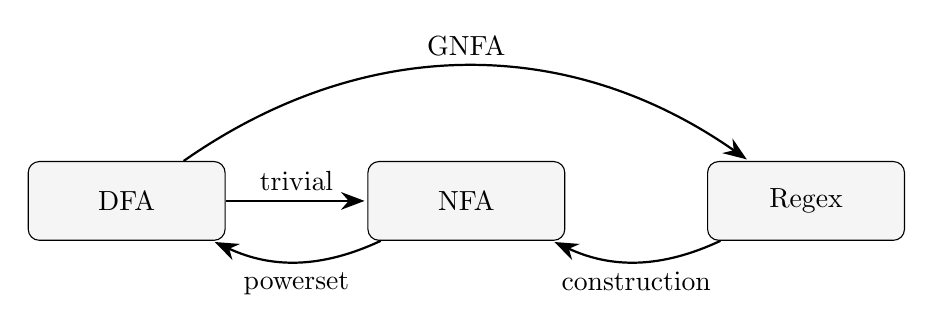
\begin{tikzpicture}[
  box/.style={draw, rounded corners, minimum width=2.5cm, minimum height=1cm, fill=black!4, align=center},
  arr/.style={-{Stealth[length=3mm]}, thick}
]
  \node[box] (dfa) {DFA};
  \node[box, right=1.8cm of dfa] (nfa) {NFA};
  \node[box, right=1.8cm of nfa] (re) {Regex};
  \draw[arr] (dfa) -- node[above] {trivial} (nfa);
  \draw[arr] (nfa) to[bend left=25] node[below] {powerset} (dfa);
  \draw[arr] (re) to[bend left=25] node[below] {construction} (nfa);
  \draw[arr] (dfa) to[bend left=35] node[above] {GNFA} (re);
\end{tikzpicture}
\end{center}

\vspace{0.8em}
Kleene's Theorem completes the circle.

\end{frame}

%------------------------------------------------
\begin{frame}{Kleene's Theorem}

We now have two ways to describe languages:
\begin{enumerate}
    \item Finite Automata (DFA/NFA)
    \item Regular Expressions (RE)
\end{enumerate}

\vspace{1em}

\textbf{Theorem (Kleene):} A language is regular if and only if some regular expression describes it.

\vspace{1em}

This implies two directions:
\begin{itemize}
    \item \textbf{Lemma 1:} If a language is described by a regular expression, it is regular (can be converted to an NFA).
    \item \textbf{Lemma 2:} If a language is regular (recognized by a DFA), it can be described by a regular expression.
\end{itemize}

\end{frame}

%------------------------------------------------
\begin{frame}{Proof of Lemma 1: RE $\rightarrow$ NFA}

We prove this using structural induction on the definition of a regular expression. 

\vspace{1em}

We first build NFAs for the base cases:
$R=a$, $R=\eps$, and $R=\emptyset$.

\vspace{1em}

Then we show how to combine them for the inductive steps:
Union, Concatenation, and Star. 
\textit{(Wait, we already proved the closure properties! We will reuse those constructions.)}

\end{frame}


%------------------------------------------------
\begin{frame}{Why Structural Induction Works Here}

A regular expression is built from smaller regular expressions.

\vspace{0.8em}
To prove every regular expression can be converted to an NFA:

\vspace{0.6em}
\begin{enumerate}
    \item Handle the atomic expressions: $a$, $\eps$, and $\emptyset$.
    \item Assume $R_1$ and $R_2$ already have NFAs.
    \item Build NFAs for $R_1\cup R_2$, $R_1R_2$, and $R_1^*$.
\end{enumerate}

\vspace{0.8em}
This follows the grammar of regular expressions exactly.

\end{frame}

%------------------------------------------------
\begin{frame}{RE to NFA: Base Cases}

\textbf{Case 1: $R = a$}

\begin{center}
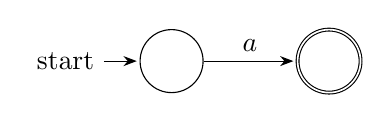
\begin{tikzpicture}[
  ->,>=Stealth,shorten >=1pt,
  node distance=2cm,
  every state/.style={minimum size=8mm},
]
\node[state, initial] (q1) {};
\node[state, accepting, right of=q1] (q2) {};
\path (q1) edge node[above] {$a$} (q2);
\end{tikzpicture}
\end{center}

\vspace{0.5em}
\textbf{Case 2: $R = \eps$}

\begin{center}
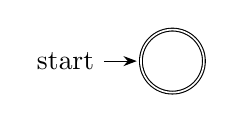
\begin{tikzpicture}[
  ->,>=Stealth,shorten >=1pt,
  every state/.style={minimum size=8mm},
]
\node[state, initial, accepting] (q1) {};
\end{tikzpicture}
\end{center}

\vspace{0.5em}
\textbf{Case 3: $R = \emptyset$}

\begin{center}
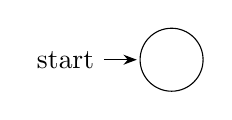
\begin{tikzpicture}[
  ->,>=Stealth,shorten >=1pt,
  every state/.style={minimum size=8mm},
]
\node[state, initial] (q1) {};
\end{tikzpicture}
\end{center}

\end{frame}

%------------------------------------------------
\begin{frame}{RE to NFA: Inductive Steps}

If $R = R_1 \cup R_2$, $R = R_1 \circ R_2$, or $R = R_1^*$, we assume we already have NFAs $N_1$ and $N_2$ for $R_1$ and $R_2$.

\vspace{1em}

We simply plug $N_1$ and $N_2$ into the constructions we proved earlier during the Closure Properties section!

\vspace{1em}
This systematic translation is often called \textbf{Thompson's Construction}.

\end{frame}

%------------------------------------------------
\begin{frame}{Example: Convert $(ab \cup a)^*$ to NFA}

Step 1: Build NFAs for $a$ and $b$.

Step 2: Concatenate them to get $ab$.

\begin{center}
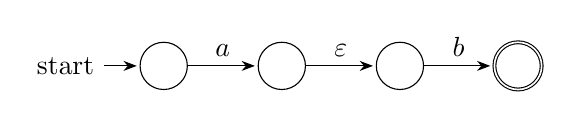
\begin{tikzpicture}[
  ->,>=Stealth,shorten >=1pt,
  node distance=1.5cm,
  every state/.style={minimum size=6mm, inner sep=0pt},
]
\node[state, initial] (q1) {};
\node[state, right of=q1] (q2) {};
\node[state, right of=q2] (q3) {};
\node[state, accepting, right of=q3] (q4) {};

\path 
(q1) edge node[above] {$a$} (q2)
(q2) edge node[above] {$\eps$} (q3)
(q3) edge node[above] {$b$} (q4);
\end{tikzpicture}
\end{center}

\end{frame}

%------------------------------------------------
\begin{frame}{Example: Convert $(ab \cup a)^*$ to NFA}

Step 3: Union with NFA for $a$ to get $(ab \cup a)$.

\begin{center}
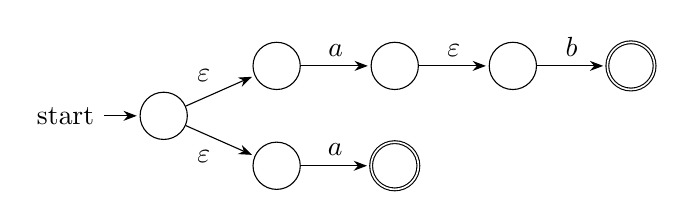
\begin{tikzpicture}[
  ->,>=Stealth,shorten >=1pt,
  node distance=1.5cm,
  every state/.style={minimum size=6mm, inner sep=0pt},
]

\node[state, initial] (q0) {};

\node[state, above right=0.2cm and 1cm of q0] (q1) {};
\node[state, right of=q1] (q2) {};
\node[state, right of=q2] (q3) {};
\node[state, accepting, right of=q3] (q4) {};

\node[state, below right=0.2cm and 1cm of q0] (p1) {};
\node[state, accepting, right of=p1] (p2) {};

\path 
(q0) edge node[above left] {$\eps$} (q1)
(q0) edge node[below left] {$\eps$} (p1)
(q1) edge node[above] {$a$} (q2)
(q2) edge node[above] {$\eps$} (q3)
(q3) edge node[above] {$b$} (q4)
(p1) edge node[above] {$a$} (p2);

\end{tikzpicture}
\end{center}

\end{frame}

%------------------------------------------------
\begin{frame}{Example: Convert $(ab \cup a)^*$ to NFA}

Step 4: Apply Star to the whole machine.

\begin{center}
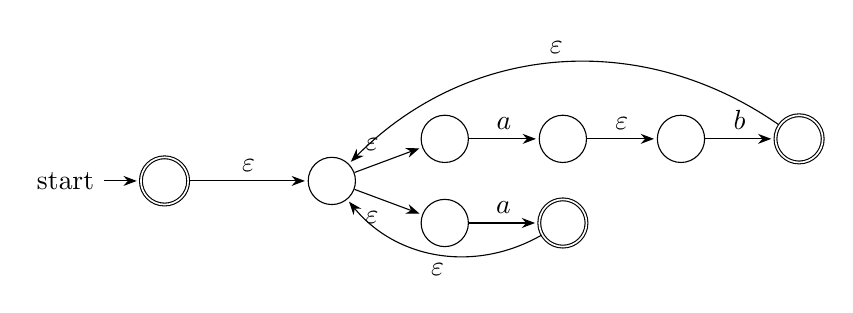
\begin{tikzpicture}[
  ->,>=Stealth,shorten >=1pt,
  node distance=1.5cm,
  every state/.style={minimum size=6mm, inner sep=0pt},
]

\node[state, initial, accepting] (start) {};

\node[state, right=1.5cm of start] (q0) {};

\node[state, above right=0.1cm and 1cm of q0] (q1) {};
\node[state, right of=q1] (q2) {};
\node[state, right of=q2] (q3) {};
\node[state, accepting, right of=q3] (q4) {};

\node[state, below right=0.1cm and 1cm of q0] (p1) {};
\node[state, accepting, right of=p1] (p2) {};

\path 
(start) edge node[above] {$\eps$} (q0)
(q0) edge node[above left] {$\eps$} (q1)
(q0) edge node[below left] {$\eps$} (p1)
(q1) edge node[above] {$a$} (q2)
(q2) edge node[above] {$\eps$} (q3)
(q3) edge node[above] {$b$} (q4)
(p1) edge node[above] {$a$} (p2)

(q4) edge[bend right=40] node[above] {$\eps$} (q0)
(p2) edge[bend left=40] node[below] {$\eps$} (q0);

\end{tikzpicture}
\end{center}
\vspace{0.2em}
\small We can easily construct an NFA for any RE.

\end{frame}


%================================================
\section{Lecture 5E: From DFA to Regular Expression}

%------------------------------------------------
\begin{frame}{Proof of Lemma 2: DFA $\rightarrow$ RE}

If a language is regular, it is recognized by a DFA. We need an algorithm to convert a DFA into a Regular Expression.

\vspace{1em}

We will do this using a new type of machine called a \textbf{Generalized Nondeterministic Finite Automaton (GNFA)}.

\vspace{1em}
A GNFA is an NFA where the transitions are labeled by \textbf{entire regular expressions}, not just single symbols or $\eps$.

\end{frame}

%------------------------------------------------
\begin{frame}{What is a GNFA?}

In a GNFA, a transition from $q_i$ to $q_j$ labeled with $R$ means: 
The machine can travel from $q_i$ to $q_j$ if it reads a block of input that matches the regular expression $R$.

\vspace{1em}

\begin{center}
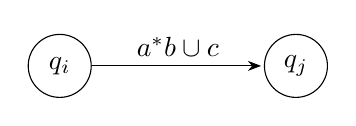
\begin{tikzpicture}[
  ->,>=Stealth,shorten >=1pt,
  node distance=3cm,
  every state/.style={minimum size=8mm},
]
\node[state] (qi) {$q_i$};
\node[state, right of=qi] (qj) {$q_j$};

\path (qi) edge node[above] {$a^*b \cup c$} (qj);
\end{tikzpicture}
\end{center}

\end{frame}


%------------------------------------------------
\begin{frame}{GNFA Transition Function}

A GNFA has a transition function of the form
\[
\delta : (Q\setminus\{q_{accept}\}) \times (Q\setminus\{q_{start}\}) \to \mathcal R,
\]
where $\mathcal R$ is the set of all regular expressions over $\Sigma$.

\vspace{0.8em}
So each allowed ordered pair of states has exactly one regular-expression label.

\vspace{0.8em}
If there is no real way to move from $p$ to $q$, the label is $\emptyset$.

\end{frame}

%------------------------------------------------
\begin{frame}{The Rules of a Sipser GNFA}

For our conversion algorithm, we enforce a strict form on the GNFA:

\begin{enumerate}
    \item The start state has transitions going \textit{to} every other state, but no transitions coming \textit{in}.
    \item There is a single accept state, which has transitions coming \textit{in} from every other state, but no transitions going \textit{out}.
    \item The start state and accept state are different.
    \item Except for the start and accept states, one arrow goes from every state to every other state, and also from each state to itself.
\end{enumerate}

\end{frame}

%------------------------------------------------
\begin{frame}{Preparing a DFA for the GNFA Algorithm}

Given a DFA, how do we force it into this strict GNFA form?

\vspace{1em}

\begin{enumerate}
    \item Add a \textbf{new start state} with an $\eps$-transition to the old start state.
    \item Add a \textbf{new single accept state} with $\eps$-transitions from all old accept states.
    \item If any required transitions are missing, add them with the label $\emptyset$.
    \item If a state has multiple parallel transitions to another state (e.g., on $a$ and on $b$), combine them using Union ($a \cup b$).
\end{enumerate}

\end{frame}


%------------------------------------------------
\begin{frame}{Why Add New Start and Accept States?}

The new start state makes sure no transition enters the start.

\vspace{0.8em}
The new accept state makes sure no transition leaves the accept state and there is only one final state.

\vspace{0.8em}
These rules simplify the algorithm: at the end, exactly two states remain and the one remaining label is the answer.

\vspace{0.8em}
Without this normalization, the final expression would require extra case handling.

\end{frame}

%------------------------------------------------
\begin{frame}{The Core Idea: State Ripping}

Once we have a GNFA, we will successively remove (``rip'') internal states one by one, while preserving the language recognized.

\vspace{1em}

When we rip a state $q_{rip}$, we must repair the transitions between all remaining pairs of states $q_i$ and $q_j$.

\vspace{1em}

Eventually, only the start state and the accept state will remain. The single transition between them will be the final Regular Expression!

\end{frame}

%------------------------------------------------
\begin{frame}{The Ripping Formula}

Suppose we want to rip state $q_{rip}$. 
For any pair of remaining states $q_i$ and $q_j$, we update the direct transition label $R(q_i, q_j)$.

\vspace{1em}

The old machine could go from $q_i$ to $q_j$ directly, OR it could go through $q_{rip}$. 

\vspace{1em}
The new label must be:

$$ R_{new}(q_i, q_j) = R_{old}(q_i, q_j) \cup \left( R(q_i, q_{rip}) \circ (R(q_{rip}, q_{rip}))^* \circ R(q_{rip}, q_j) \right) $$

\end{frame}

%------------------------------------------------
\begin{frame}{Visualizing the State Rip}
\small

\textbf{Before ripping $q_{rip}$:}

\begin{center}
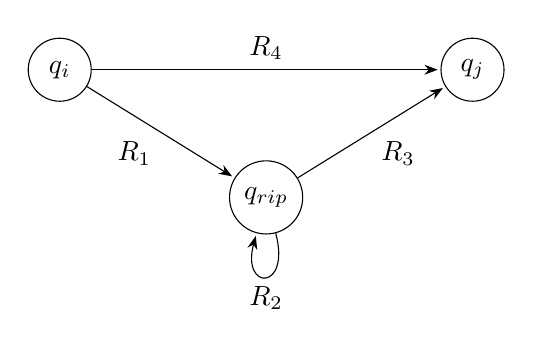
\begin{tikzpicture}[
  ->,>=Stealth,shorten >=1pt,
  node distance=2.5cm,
  every state/.style={minimum size=8mm},
]
\node[state] (qrip) {$q_{rip}$};
\node[state, above left=1cm and 2cm of qrip] (qi) {$q_i$};
\node[state, above right=1cm and 2cm of qrip] (qj) {$q_j$};

\path 
(qi) edge node[above] {$R_4$} (qj)
(qi) edge node[below left] {$R_1$} (qrip)
(qrip) edge[loop below] node {$R_2$} ()
(qrip) edge node[below right] {$R_3$} (qj);
\end{tikzpicture}
\end{center}

\vspace{0.5em}

\textbf{After ripping $q_{rip}$:}

\begin{center}
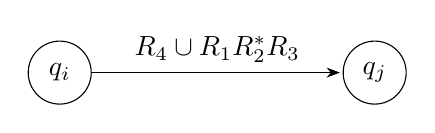
\begin{tikzpicture}[
  ->,>=Stealth,shorten >=1pt,
  node distance=4cm,
  every state/.style={minimum size=8mm},
]
\node[state] (qi) {$q_i$};
\node[state, right of=qi] (qj) {$q_j$};

\path 
(qi) edge node[above] {$R_4 \cup R_1 R_2^* R_3$} (qj);
\end{tikzpicture}
\end{center}

\end{frame}


%------------------------------------------------
\begin{frame}{Different Regexes Can Describe the Same Language}

Regular expressions are not unique.

\vspace{0.8em}
For strings ending in $1$, all of the following describe the same language:
\[
(0\cup1)^*1,
\]
\[
0^*1(1\cup 00^*1)^*,
\]
\[
\Sigma^*1.
\]

\vspace{0.8em}
The GNFA algorithm gives a correct expression, not necessarily the prettiest expression.

\end{frame}

%------------------------------------------------
\begin{frame}{Summary of Kleene's Theorem}

We have shown a complete lifecycle:

\begin{enumerate}
    \item \textbf{Regular Expressions} precisely define patterns algebraically.
    \item We can convert any RE into an \textbf{NFA} (using base structures and closure properties).
    \item Every NFA is equivalent to a \textbf{DFA} (using powerset construction).
    \item We can convert any DFA back into a \textbf{Regular Expression} (using GNFA and state ripping).
\end{enumerate}

\vspace{1em}
\pause
Therefore, DFAs, NFAs, and Regular Expressions all describe exactly the same class of languages: \textbf{The Regular Languages}.

\end{frame}

\end{document}
